\documentclass[conference]{IEEEtran}
\IEEEoverridecommandlockouts

\usepackage{cite}
\usepackage{amsmath,amssymb,amsfonts}
\usepackage{graphicx}
\usepackage{booktabs}
\usepackage{url}
\usepackage{hyperref}
\hypersetup{hidelinks}
\usepackage{balance}
\usepackage{tikz}
\usetikzlibrary{arrows.meta}
\tikzset{
  sm/.style={draw, rounded corners=2pt, font=\footnotesize, align=center,
             inner sep=3pt, minimum height=6.2mm, line width=0.6pt},
  sml/.style={font=\scriptsize, fill=white, inner sep=1.4pt, align=center},
  arr/.style={->, >=Stealth, line width=0.6pt}
}

\def\CoRAL{CoRAL}
\def\otterk{\texttt{otter\_k}}
\def\xudrone{\texttt{xudrone}}

\begin{document}

\title{CoRAL: Language-Specified Joint Missions\\
of an Autonomous Surface Vehicle\\
and an Autonomous Underwater Vehicle}

\author{\IEEEauthorblockN{Jnaneshwar Das}
\IEEEauthorblockA{\textit{Earth Innovation Hub / DREAMS Lab}\\
\textit{Arizona State University}\\
Tempe, Arizona, USA\\
jdas@earthinnovationhub.org}
\thanks{Draft for IEEE ICRA style. Results are from the Kiwanis Gazebo twin, not a field trial.}}

\maketitle

\begin{abstract}
We describe \CoRAL{}, a closed loop that turns a spoken joint mission into typed behaviours for a surface vehicle and an underactuated autonomous underwater vehicle (AUV) in a Gazebo twin of Kiwanis Lake, Tempe. The pair is \otterk{}, a digital twin of a catamaran autonomous surface vehicle (ASV) designed by the DREAMS Lab, and \xudrone{}, a digital twin of an AUV designed by the same lab, whose four thrusters push only along the hull. The AUV can pitch and yaw, and it cannot roll or sway. The demonstration mission is one sentence: undock, fly through a hoop, and rendezvous with the boat. A phrase recognizer, backed by a language model for open wording, compiles that sentence into detach, hoop, and rendezvous. A behaviour node runs one step at a time and keeps the AUV armed between steps.

The same underactuation explains the control result. A time-indexed trajectory, inherited from a helical tracker, asks the hull to chase a moving point. At the drag-model cruise the brake spiked; at a slower pace the hull fell behind the reference and the heading command collapsed. Straight legs now use line-of-sight (LOS) guidance with no clock: the hull turns in place onto the line, a surge loop ramps and brakes, and pitch and heading close the depth and cross-track errors. In the twin, an 8\,m leg that began 173$^\circ$ off the line finished in 8.4\,s with thrust at most 0.24 of full scale and depth error at most 0.16\,m. The joint mission then passed the hoop 0.10\,m from the opening centre and latched under the boat. We report these as single demonstration runs.
\end{abstract}

\begin{IEEEkeywords}
Marine robotics, autonomous underwater vehicles, autonomous surface vehicles, line-of-sight guidance, underactuated control, language-conditioned planning, digital twin
\end{IEEEkeywords}

\section{Introduction}
\label{sec:intro}

A joint surface--underwater mission is easy to say and hard to fly. ``Undock, fly through the hoop, and rendezvous with the boat'' names three different problems: releasing a latched AUV, steering a body that cannot move sideways through a small opening, and docking that body under a moving hull. Each problem has its own sensing, its own acceptance test, and its own way of failing. A language model that emits a free-form trajectory does not own any of those tests. A controller that treats the AUV as a fully actuated point mass does not own the vehicle.

This paper states that split and the system we built around it. \CoRAL{} is the aquatic half of a lab stack that already flies a multirotor and a ground rover from the same language interface. On the water the vehicles are \otterk{}, a digital twin of a catamaran autonomous surface vehicle (ASV) designed by the DREAMS Lab, and \xudrone{}, a digital twin of an AUV designed by the DREAMS Lab, docked under it. Both live in one Gazebo world of Kiwanis Lake. The operator's sentence becomes a short list of typed steps. Each step is a behaviour with a pass/fail event. The next step starts only when the current one ends, and the AUV stays armed across that handoff so the mission does not fall out of offboard control.

The control contribution is narrower than the system. \xudrone{} is steered like a quadrotor lying on its side: the force the guidance wants is turned into a hull direction, and the thrust is the part of that force along the nose. That construction is a good fit for a curve whose acceleration is known, and a poor fit for a straight leg whose reference is a function of time. A carrot that moves on a clock pulls a lagging hull off the line, toward the carrot, and a carrot that brakes faster than the hull can stop pitches the nose. We replace the timed carrot on straight swims with LOS guidance \cite{fossen2011,lekkas2014}. Heading and pitch steer onto the line. Speed is a separate command. There is no time parameter for the lag to accumulate in.

The paper makes three claims, each limited to the digital twin.
\begin{enumerate}
\item A joint ASV--AUV mission can be compiled from one sentence into a fixed behaviour chain whose order does not depend on the spoken order, while open wording still goes to a planner.
\item For this hull, waypoint legs should be path followers, not time-parameterized trajectory trackers. LOS swim is the first behaviour moved across that line.
\item The hoop-and-dock chain is executable end to end: the AUV releases, crosses an authored opening, and latches under the boat on a centreline glide that does not orbit the nest.
\end{enumerate}

Section~\ref{sec:related} places the work. Section~\ref{sec:world} describes the aquatic world and the robot team. Section~\ref{sec:coral} is the language and behaviour machine. Section~\ref{sec:control} is the hull law and the LOS swim. Section~\ref{sec:mission} is the hoop and the rendezvous. Section~\ref{sec:results} reports the runs. Section~\ref{sec:conclusion} states what is not yet shown.

\section{Related work}
\label{sec:related}

Cooperative ASV--AUV navigation is an established problem. An ASV can carry a better navigation fix, a deck marker, and a dock, while the AUV works under the surface. Anand's thesis studies that split in the OpenUAV simulator and holds an AUV several metres under a marker on the ASV \cite{anand2020}. Kiwanis Lake is about 2.4\,m deep, so the same idea cannot use a 5\,m standoff. Our follow distance under the deck tag is 1\,m, and the dock is a weld under the hull rather than a station-keep at depth. The sensing is also different: we keep a Gazebo world and AprilTag fiducials \cite{olson2011} on the deck, the pontoon sterns, and a submerged cube, instead of the Unity front end used in that thesis.

Guidance for vehicles that cannot sway is classical LOS path following \cite{fossen2011,lekkas2014}. The heading command is the path angle minus the bearing of the cross-track error over a look-ahead distance. Integral LOS rejects a constant sideslip. Our hull has no sideslip actuator at all, and it also has to change depth by pitching, because the same thrusters that surge also provide the only vertical force once the nose is down. The guidance in Section~\ref{sec:control} is therefore LOS in heading and in pitch, plus a surge speed loop. We do not claim a new LOS law. We claim that this vehicle should use one on waypoint legs, and we show what the timed alternative did on the same hull.

Language-conditioned robot stacks usually stop at a plan: a model emits waypoints or code, and a separate controller tracks them. That split is right when the controller's assumptions match the vehicle. It fails when the plan is a clocked curve and the vehicle can only push along its nose. \CoRAL{} keeps the split, but the plan is a list of behaviours that already contain the vehicle's constraints. Fixed phrases cover the missions we are willing to fly without review. A language model covers the rest, and its output is still the same typed steps.

\section{Aquatic world and robot team}
\label{sec:world}

\subsection{The lake}
The Gazebo world replaces an oversized rectangular lake with a shoreline taken from Kiwanis Lake in Tempe, Arizona. The published lake is about 13 acres, with a maximum depth of about 8\,ft. The model origin is the shoreline polygon's centroid. The bed is a visual bowl, 1\,m at the shore and 10\,m at the deepest point. There is no bathymetric survey in the mesh, and the props (hoop, tag cube, rocks, buoys, pier) are not solid. Buoyancy is a density field below the plane $z=0$, not a free-surface mesh. Both vehicles spawn at the origin: the AUV a metre down, the boat on the surface. The twin is a sandbox. A separate twin of the same boat on Tempe Town Lake is left untouched.

The world is large enough for the behaviours we care about and small enough that a missed depth command hits the bowl. A vertical loop is clamped above that floor. The hoop sits at the midpoint of a 9.25\,m water column. The bed tag cube sits on the bottom. These are authored landmarks, not detections of the real lake.

\subsection{The surface vehicle}
\otterk{} is a digital twin of a catamaran ASV designed by the DREAMS Lab. The boat is about the size of a Heron and runs PX4 in the same simulator as the AUV. Each pontoon is 1.20\,m long and 0.24\,m in diameter, and the pontoon centres are 0.76\,m apart, so the boat is 1.20\,m long and 1.00\,m across. The hull mass is 28\,kg. It is the dock, the moving frame for rendezvous, and a vehicle with its own behaviours: a surface goto and a survey. It has no camera in this world. The AUV is the only eye. Three AprilTags face the AUV. Tag 10, 0.40\,m, is centred on the underside of the deck and is the nest marker for station-keeping and docking. Tags 11 and 12, 0.24\,m, sit on the pontoon sterns and face aft, so the AUV's front camera can see them on the approach. A latch weld accepts the AUV near the boat origin, on the midline between the pontoons, within 0.6\,m and about 30$^\circ$ of attitude error.

\subsection{The underwater vehicle}
\xudrone{} is a digital twin of an AUV designed by the DREAMS Lab. The pressure hull is a tube 0.30\,m long and 0.22\,m in diameter. Four thrusters sit in a square at the stern so that every rotor pushes along the hull axis. That stern arrangement is related to the HippoCampus micro-AUV \cite{hackbarth2015}, and this hull was designed independently. Each thruster is limited to 36\,N, so full forward thrust is 144\,N. Pitch and yaw are differential thrust on a 0.14\,m arm. Roll commands produce no motor output; ballast keeps the hull upright. The hull and its sensor and rotor links mass 13.666\,kg and displace 13.70\,kg, so the vehicle is about 0.3\,N light and rests awash rather than sinking. Body-frame drag is modelled as $1.2v + 3v^{2}$ newtons along the nose and a much larger quadratic term laterally and vertically. That drag is why a sideways force is the wrong thing to ask for: the hull will not crab, and the force has to be turned into a heading.

Three cameras look along the mission. The front camera serves the hoop, the stern tags, and the operator's video. The nadir camera sees the bed tag once the hull is over it. The upward camera, on the crown and pitched down, sees deck tag 10 during the dock. A downward range and a barometer feed the estimator. The control pose is that estimate, with Gazebo as a check: a tick whose estimate is stale or far from the simulator flies the simulator pose and records the miss.

The actuation constraint is the one that organises the rest of the paper. Any commanded force $\mathbf{f}$ is realised by pointing the hull axis $\mathbf{x}_{b}$ along a feasible direction $\mathbf{d}$ and commanding the thrust
\begin{equation}
T = \mathrm{sat}\!\left(\mathbf{f}\cdot\mathbf{x}_{b} / F_{\max}\right),
\label{eq:thrust}
\end{equation}
with $F_{\max}=144\,\mathrm{N}$. Pitch is limited on cruise behaviours, 45$^\circ$ in general and tighter near the boat, because an unlimited nose-down command dives the vehicle out of the camera's target. A small force behind the nose backs the hull up. A large one turns it around. There is no sideways channel to absorb a guidance error.

\section{From a sentence to a behaviour}
\label{sec:coral}

Fig.~\ref{fig:stack} is the whole path. Three web frontends share one operator: the DeepGIS search page, its WebXR cockpit, and the robot panel already used for the lab's other vehicles. The panel takes a sentence and a callsign. A phrase the recognizer knows becomes typed steps with no language model. Open wording goes to the model, which may emit only those same steps. \CoRAL{} then runs one step. In the aquatic twin a ROS~2 behaviour publishes the offboard setpoint, PX4 flies it, and Gazebo is the Kiwanis world that holds both robots. Video and status return to the pages. No stage emits raw thrust.

\begin{figure*}[t]
\centering
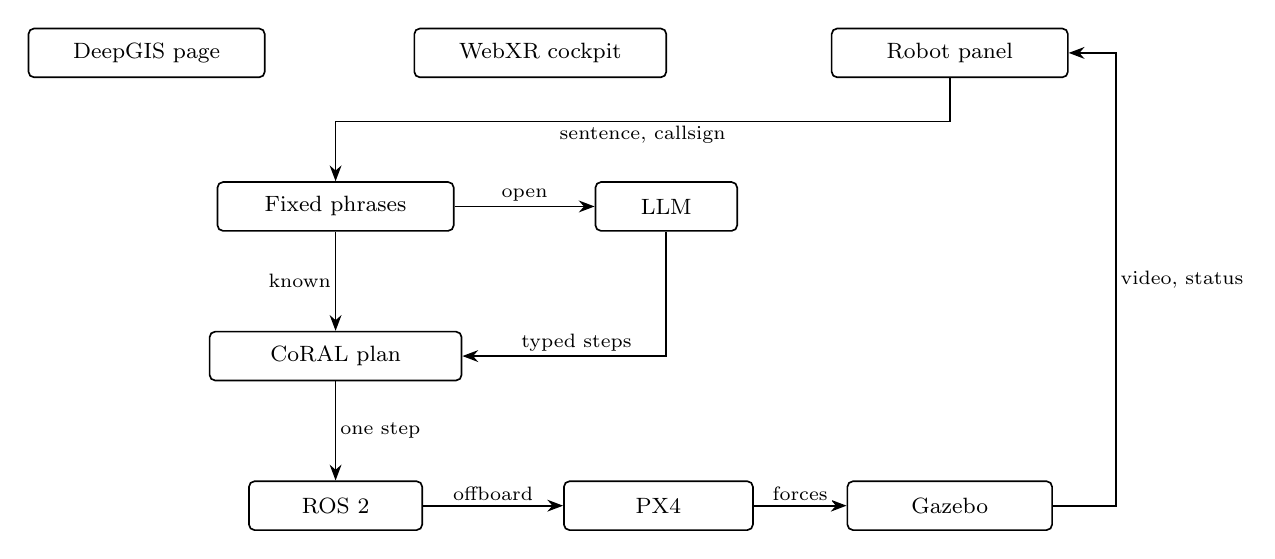
\begin{tikzpicture}
  \node[sm, minimum width=30mm] (page) at (0,0) {DeepGIS page};
  \node[sm, minimum width=32mm] (xr) at (5.0,0) {WebXR cockpit};
  \node[sm, minimum width=30mm] (panel) at (10.2,0) {Robot panel};
  \node[sm, minimum width=30mm] (phr) at (2.4,-1.95) {Fixed phrases};
  \node[sm, minimum width=18mm] (llm) at (6.6,-1.95) {LLM};
  \node[sm, minimum width=32mm] (plan) at (2.4,-3.85) {CoRAL plan};
  \node[sm, minimum width=22mm] (ros) at (2.4,-5.75) {ROS 2};
  \node[sm, minimum width=24mm] (px4) at (6.5,-5.75) {PX4};
  \node[sm, minimum width=26mm] (gz) at (10.2,-5.75) {Gazebo};
  \draw[arr] (panel.south) -- ++(0,-0.55) coordinate (sent)
    -- node[sml, below] {sentence, callsign} (phr.north |- sent) -- (phr.north);
  \draw[arr] (phr) -- node[sml, above] {open} (llm);
  \draw[arr] (phr) -- node[sml, left] {known} (plan);
  \draw[arr] (llm.south) |- node[sml, above, pos=0.72] {typed steps} (plan.east);
  \draw[arr] (plan) -- node[sml, right] {one step} (ros);
  \draw[arr] (ros) -- node[sml, above] {offboard} (px4);
  \draw[arr] (px4) -- node[sml, above] {forces} (gz);
  \draw[arr] (gz.east) -- ++(0.8,0) coordinate (side)
    -- node[sml, right] {video, status} (side |- panel.east) -- (panel.east);
\end{tikzpicture}
\caption{The stack around the aquatic twin. The search page and the WebXR cockpit are the other web frontends; the sentence is entered on the robot panel. A known phrase skips the language model. The model, when it is called, returns typed steps rather than thrust. ROS~2, PX4, and Gazebo are one simulator: the behaviours, the offboard autopilots, and the Kiwanis world with \otterk{} and \xudrone{}.}
\label{fig:stack}
\end{figure*}

\subsection{What the operator says}
The operator interface is the same one used for the lab's other vehicles: a sentence, a callsign, and a status channel. For this pair the callsigns share one simulator. A sentence may name either vehicle. The aquatic behaviours that matter for the joint mission are:

\begin{itemize}
\item \textbf{dock}: attach or detach the weld;
\item \textbf{swim}: one straight AUV leg, compass, world, or along the current heading;
\item \textbf{hoop}: find the authored ring and pass through it;
\item \textbf{rendezvous}: glide under \otterk{} and latch;
\item \textbf{track}: hold about 1\,m under the deck tag without latching;
\item \textbf{approach\_tag}, \textbf{coverage}, \textbf{shape}, \textbf{helix}: search, survey, geometric curves, and the original helix.
\end{itemize}

Boat \texttt{goto} and \texttt{survey} run on \otterk{}. A shared busy lock means one behaviour owns the pair at a time.

\subsection{Fixed phrases before the planner}
Some sentences are missions we have already decided how to fly. Those are recognized before the language model, in a fixed order: a stop, then the joint tour, then search-then-dock, then approach-then-dock, then a lone search or rendezvous, then other direct behaviours, and only then the planner.

The tour is the sentence this paper is about. ``Undock, fly through the hoop, and rendezvous with \otterk{}'' compiles to detach, hoop, rendezvous, in that order, whatever order the clauses were spoken. If the sentence also asks to approach the bed tag, that search is inserted; if it does not, the tag approach is left out. Earlier, a dock phrase that also mentioned the hoop could drop the hoop and send the vehicle straight to the nest. The recognizer now refuses to treat a hoop sentence as a pure dock. A new instruction aborts the step it supersedes instead of leaving the old one flying.

Open wording still goes to the planner. The planner's vocabulary is the same typed steps, including a stop condition such as ``until a tag is detected.'' An AUV compass instruction becomes a swim, not a helix. A shape sentence becomes a geometric path. The planner is asked for a short JSON plan, not a chain of thought long enough to come back empty. A duplicate completion event does not start the next step twice.

This split is deliberate. The tour is a demonstration with a known safe order. The planner is for legs we can check one at a time. Neither path emits raw thrust.

\subsection{The behaviour machine}
Inside the twin, one node subscribes to a command topic and publishes events: accepted, done, failed, aborted. A bridge outside the twin presents those as the mission-supervisor topics the rest of the lab already uses, and it maps high-level commands onto the aquatic types. Reset restarts the simulator even if a behaviour is busy.

While a step runs, the AUV is in offboard mode and armed. When the step finishes, the process does not disarm. It holds the point where it ended and hands a baton to a hold process: the hold process's identity, and the depth-integrator state. The next behaviour asks for the baton and starts publishing on the following tick. The gap is about one control period. PX4's offboard-loss timeout is 1\,s, so a clean handoff does not drop the vehicle out of the mode. The hold process disarms on abort, reset, dock, or a long timeout. Docking is the step that is allowed to end the free swim, because the weld then owns the hull.

Failed steps are events, not silences. A hoop that misses can be told to hold and continue, so a rendezvous later in the plan still runs. A failed dock does not leave the plan hanging. The status channel reports whether the AUV is holding, whether the latch is attached, and which phase is active. Fig.~\ref{fig:plan} is that plan machine. Fig.~\ref{fig:auv} is the process that flies one step and hands the armed vehicle to the next.

\begin{figure}[t]
\centering
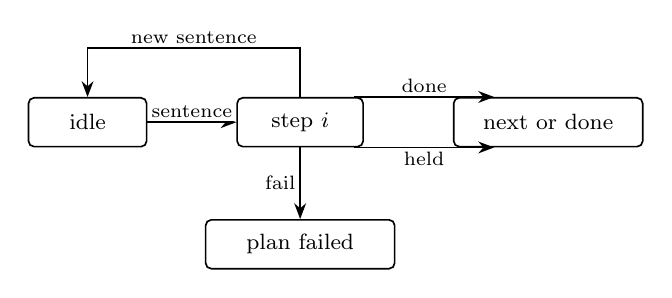
\begin{tikzpicture}
  \node[sm, minimum width=15mm] (idle) at (0,0) {idle};
  \node[sm, minimum width=16mm] (step) at (2.7,0) {step $i$};
  \node[sm, minimum width=24mm] (next) at (5.85,0) {next or done};
  \node[sm, minimum width=24mm] (fail) at (2.7,-1.55) {plan failed};
  \draw[arr] (idle) -- node[sml, above] {sentence} (step);
  \draw[arr] (step.25) -- node[sml, above] {done} (next.155);
  \draw[arr] (step.335) -- node[sml, below] {held} (next.205);
  \draw[arr] (step) -- node[sml, left] {fail} (fail);
  \draw[arr] (step.north) -- ++(0,0.62) coordinate (hi)
    -- node[sml, above] {new sentence} (idle.north |- hi) -- (idle.north);
\end{tikzpicture}
\caption{Plan execution. Done moves to the next step, or finishes the plan. A hoop miss that was told to hold does the same, and the vehicle stays armed. Any other failure ends the plan. A new sentence aborts the step that is running.}
\label{fig:plan}
\end{figure}

\begin{figure}[t]
\centering
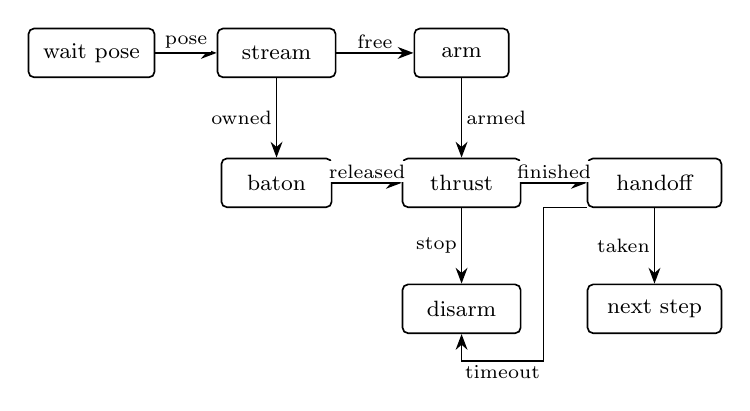
\begin{tikzpicture}
  \node[sm, minimum width=16mm] (wait) at (0,0) {wait pose};
  \node[sm, minimum width=15mm] (stream) at (2.35,0) {stream};
  \node[sm, minimum width=12mm] (arm) at (4.7,0) {arm};
  \node[sm, minimum width=14mm] (baton) at (2.35,-1.65) {baton};
  \node[sm, minimum width=15mm] (thrust) at (4.7,-1.65) {thrust};
  \node[sm, minimum width=17mm] (hand) at (7.15,-1.65) {handoff};
  \node[sm, minimum width=15mm] (off) at (4.7,-3.25) {disarm};
  \node[sm, minimum width=17mm] (nxt) at (7.15,-3.25) {next step};
  \draw[arr] (wait) -- node[sml, above] {pose} (stream);
  \draw[arr] (stream) -- node[sml, above] {free} (arm);
  \draw[arr] (stream) -- node[sml, left] {owned} (baton);
  \draw[arr] (arm) -- node[sml, right] {armed} (thrust);
  \draw[arr] (baton) -- node[sml, above] {released} (thrust);
  \draw[arr] (thrust) -- node[sml, above] {finished} (hand);
  \draw[arr] (thrust) -- node[sml, left] {stop} (off);
  \draw[arr] (hand) -- node[sml, left] {taken} (nxt);
  \draw[arr] (hand.200) -- ++(-0.55,0) coordinate (hw)
    -- ++(0,-1.95) coordinate (low)
    -- node[sml, below] {timeout} (off.south |- low) -- (off.south);
\end{tikzpicture}
\caption{One behaviour process, read from the top. A free vehicle is armed, then flies. If another process already holds it, this one waits for the baton and never disarms. The finished step holds its point until the next process takes over. Stop and handoff timeout both disarm.}
\label{fig:auv}
\end{figure}

\section{Control of a body-x hull}
\label{sec:control}

\subsection{The force loop}
Most behaviours share one controller. A reference supplies a desired position, velocity, and, when it knows it, acceleration, in a path frame fixed at the pose where thrust started. The world force is
\begin{equation}
\begin{aligned}
\mathbf{f} = {} & m\big(k_{v}(\mathbf{v}_{\mathrm{cmd}}-\mathbf{v}) + \mathbf{a}_{\mathrm{ff}}\big) \\
& + \mathbf{d}(\mathbf{v}_{\mathrm{cmd}}) - b\,\mathbf{e}_{z},
\end{aligned}
\label{eq:force}
\end{equation}
where $\mathbf{v}_{\mathrm{cmd}}$ is the reference velocity plus a saturated position correction, $\mathbf{d}$ is drag at that command, and $b$ is the small net buoyancy plus a depth integrator that runs only near the setpoint. The hull direction tracks $\mathbf{f}$, with the pitch limit and the backup rule of Section~\ref{sec:world}. Equation~\eqref{eq:thrust} is the thrust.

This is the right law for a helix, a figure-eight, an orbit, or a vertical loop, where the path acceleration is the feedforward, and for holding a point under the boat. It is the wrong law for ``swim 8\,m west'' when the reference is a point that moves with time. The hull can fall behind that point. The position correction then points at the carrot rather than along the line. If the carrot brakes, $\mathbf{a}_{\mathrm{ff}}$ and the velocity error point backward while the hull is still fast, and the nose follows them down.

We tried to fix the timed swim by changing only its speed. At the speed where 85\% of full thrust balances body-x drag, about 6.2\,m/s, the brake spiked to about 50\,N and the nose reached $-37^\circ$. At 2\,m/s and at 0.35\,m/s the feedforward was too small: the hull fell about 1.3\,m behind the carrot, the progress gate slowed the clock, and the horizontal force dropped under the 1.5\,N threshold that is willing to change heading. There is no single pace at which a clocked point is a good reference for this hull. Shapes and coverage still use the timed reference, with a progress gate that slows the clock past 0.6\,m of error and stops it at 2\,m. Swim does not.

\subsection{Line-of-sight swim}
\label{sec:los}
A swim is two waypoints in the world: the pose at thrust-on, and the compass or heading offset, at constant depth unless a depth was requested. \texttt{LosGuide} takes the waypoint list, the pose, the yaw, and the measured nose elevation. It returns a heading, a pitch, a speed, and a unit direction. It has no time argument.

On the current leg, with the hull at along-track coordinate $s$ and cross-track error $e$, the heading is the standard LOS command
\begin{equation}
\psi = \chi - \mathrm{atan2}(e, \Delta),
\label{eq:los}
\end{equation}
where $\chi$ is the leg course and the look-ahead $\Delta$ grows from 1.5\,m to 4\,m with speed. Depth uses the same form against a shorter look-ahead, 1.0\,m to 2.5\,m, and the resulting flight-path angle is clamped to the pitch limit. The sign flips when the hull has passed the end and must back up along the line, so reverse thrust still reduces the error.

The direction sent to the attitude loop is not the raw LOS heading when that heading is behind the nose. An aim more than 90$^\circ$ off the hull has no unique rotation axis, and the attitude loop can pitch over instead of yawing around. The aim is therefore held within 75$^\circ$ of the current heading, and the pitch command is held level until the heading error is inside 30$^\circ$. Inside that cone the surge command is released. Outside it the speed command is zero: the hull turns in place.

Speed is a first-order reference, not a position deadline. It ramps at 1\,m/s$^{2}$ and is allowed to fall at 1.5\,m/s$^{2}$. On the last leg it is limited by a constant-deceleration brake at 0.6\,m/s$^{2}$ and by a proportional cap in the last metre, so the command is zero at the waypoint. An interior corner slows the arrival speed in proportion to the turn. The thrust loop cancels drag at the reference speed and closes the error between that speed and the speed along the nose:
\begin{equation}
f_{x} = m\big(k_{v}(u_{\mathrm{ref}}-u) + a_{\mathrm{ref}}\big) + d_{x}(u_{\mathrm{ref}}).
\label{eq:surge}
\end{equation}
A buoyancy term along the nose is removed. The same thrust limit as \eqref{eq:thrust} applies.

On the twin the nose rides several degrees below the pitch command while the hull is moving. An integrator on the elevation error, active only above 0.3\,m/s and only while the heading is inside the surge cone, learns that bias up to 12$^\circ$. Without it, an 8\,m west leg settled half a metre below the line. With it, the depth error on the next leg of that kind stayed within 0.16\,m.

If the hull stops on the line but outside the 0.35\,m arrival ball, LOS has nothing left to do: at zero speed, pitch no longer moves the vehicle vertically, and a pure cross-track correction would demand a sideways force. The swim then hands the end point to the force loop for at most 10\,s. That settle is what closed a 3\,m south leg that stopped 0.52\,m to the side. Fig.~\ref{fig:swim} is this mode switch. There is still no clock.

\begin{figure}[t]
\centering
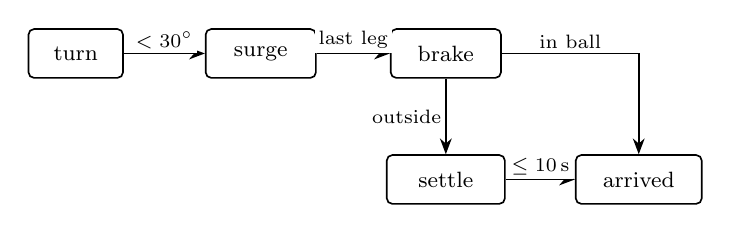
\begin{tikzpicture}
  \node[sm, minimum width=12mm] (turn) at (0,0) {turn};
  \node[sm, minimum width=14mm] (surge) at (2.35,0) {surge};
  \node[sm, minimum width=14mm] (brake) at (4.7,0) {brake};
  \node[sm, minimum width=15mm] (settle) at (4.7,-1.6) {settle};
  \node[sm, minimum width=16mm] (done) at (7.15,-1.6) {arrived};
  \draw[arr] (turn) -- node[sml, above] {$<30^\circ$} (surge);
  \draw[arr] (surge) -- node[sml, above] {last leg} (brake);
  \draw[arr] (brake) -- node[sml, left] {outside} (settle);
  \draw[arr] (settle) -- node[sml, above] {$\leq 10$\,s} (done);
  \draw[arr] (brake.east) -- node[sml, above] {in ball}
    (done.north |- brake.east) -- (done.north);
\end{tikzpicture}
\caption{Line-of-sight swim. While the heading error is larger than $30^\circ$ the speed command stays zero, so the hull yaws before it moves. The last leg brakes. Inside the arrival ball the step ends. Outside it, the force loop holds the end point for at most 10\,s.}
\label{fig:swim}
\end{figure}

The old timed swim remains available behind a switch, so the two guidances can be compared on the same binary. The unstated swim pace is still the 6.2\,m/s drag-model cruise. LOS never treats that number as a position rate. On a short leg the brake limit keeps the speed near 2.5\,m/s.

\subsection{What stays on the force loop}
LOS is the wrong tool for holding a point, for the last metre of a dock, and for a visual servo on a tag. Those behaviours keep \eqref{eq:force}. The helix and the geometric shapes keep it because their reference is a curve with a meaningful acceleration. Coverage lawnmowers and the rendezvous transit are polylines and are the next candidates to move. The hoop is a special case: it already limits speed so that depth and lateral error close before the plane, and it picks nose-down or nose-up thrust from the commanded velocity rather than from the force, after a pitch limit cycle in the dive.

\section{The joint mission}
\label{sec:mission}

\subsection{Release}
The mission starts with the AUV welded under the boat. Detach is a latch command, not a swim. The behaviour node reports the latch state and will not start a free-swim behaviour that the latch would fight. After detach, the baton rules of Section~\ref{sec:coral} apply: the hoop starts armed.

\subsection{The hoop}
The hoop is a 1\,m vertical ring, authored at a fixed pose, with its opening along east--west. The rim is not tagged. The AUV searches a grid centred on the dock until orange pixels form a ring whose centre lies within 1.25\,m horizontally and 0.85\,m in depth of the authored hoop. A closed ring that fails that test does not start an approach. Range during search comes from the ellipse of the orange blob and the ring's known outer diameter.

Once the ring is locked, the pass is one pursuit reference rather than a vision chase of the image centre. Waiting for the ring to reach the centre of a shallow approach never fired, and the resulting lead flew through and below the opening. Short of the plane, forward speed is capped so the depth error and the lateral error close first. On the line the cruise is at most 0.32\,m/s, with a short pursuit lead, and the nose is free: locking the yaw would drop the lateral force, and the hull cannot sideslip. A pass requires two geometric facts, not a camera crop. One sample must lie inside the authored opening, within 0.40\,m of the centre, and the hull must later arrive within about 0.6\,m of the exit point that was frozen at entry. Time spent in the ring does not count. A miss goes around beside the ring rather than reversing through it. When a rendezvous follows in the plan, a failed pass holds and the plan continues.

\subsection{Rendezvous and dock}
The failure mode this glide is built to avoid is an orbit. A body-x hull told to chase a point under the nest circles that point. The terminal guidance therefore does not pursue a point. It flies the boat's centreline.

The approach begins on an aft station, 6\,m behind the nest. Heading on the glide is a bounded LOS command in the boat frame: the boat's yaw, minus the bearing of the lateral error over a look-ahead, clamped so a large miss cannot command more than a set intercept angle. The front camera's fixes on the stern tags and the deck tag correct the boat pose the glide flies on. The correction is a horizontal offset on the boat's prior, weighted by inverse range, limited per update and in total, and held when no tag is in view. Guidance uses the corrected pose. The boat-velocity estimate used by the controller stays on the prior, so a vision jump is not a velocity spike.

Capture is a short leg through the weld sphere, 0.25\,m under the nest, along the boat heading, at low speed. The hull may enter it only when it is near the end of the glide, close to the centreline, and already slow. Otherwise the flare keeps flying. The latch command is sent from any stage once the weld gate has held for a quarter second, not only from a dedicated dock state. Overshooting the sphere, drifting more than a metre off the line, or staying in capture too long returns the hull to the start of the glide. More than three returns fail the behaviour. Fig.~\ref{fig:skills} is the hoop and this rendezvous. Both count a retry and both stop after three.

\begin{figure*}[t]
\centering
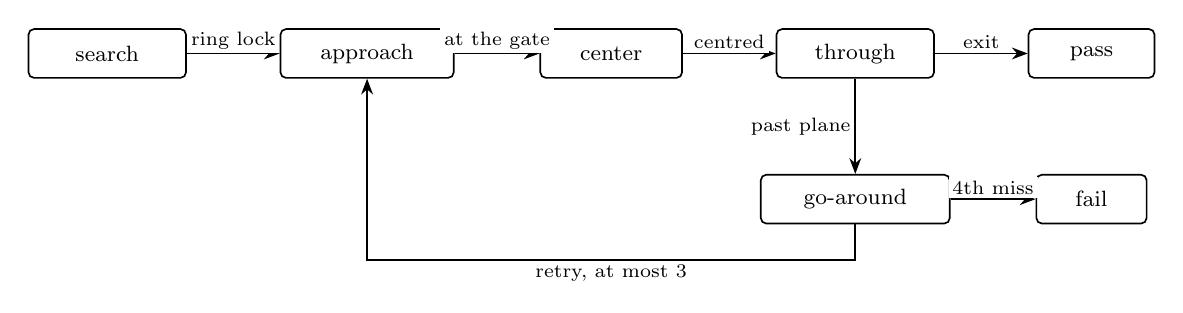
\begin{tikzpicture}
  \node[sm, minimum width=20mm] (search) at (0,0) {search};
  \node[sm, minimum width=22mm] (appr) at (3.3,0) {approach};
  \node[sm, minimum width=18mm] (center) at (6.4,0) {center};
  \node[sm, minimum width=20mm] (thru) at (9.5,0) {through};
  \node[sm, minimum width=16mm] (pass) at (12.5,0) {pass};
  \node[sm, minimum width=24mm] (ga) at (9.5,-1.85) {go-around};
  \node[sm, minimum width=14mm] (fail) at (12.5,-1.85) {fail};
  \draw[arr] (search) -- node[sml, above] {ring lock} (appr);
  \draw[arr] (appr) -- node[sml, above] {at the gate} (center);
  \draw[arr] (center) -- node[sml, above] {centred} (thru);
  \draw[arr] (thru) -- node[sml, above] {exit} (pass);
  \draw[arr] (thru) -- node[sml, left] {past plane} (ga);
  \draw[arr] (ga) -- node[sml, above] {4th miss} (fail);
  \draw[arr] (ga.south) -- ++(0,-0.45) coordinate (hlow)
    -- node[sml, below] {retry, at most 3} (appr.south |- hlow) -- (appr.south);
\end{tikzpicture}

\vspace{3.5mm}
{\footnotesize (a) Hoop. A miss goes beside the ring and tries the approach again.}

\vspace{4mm}
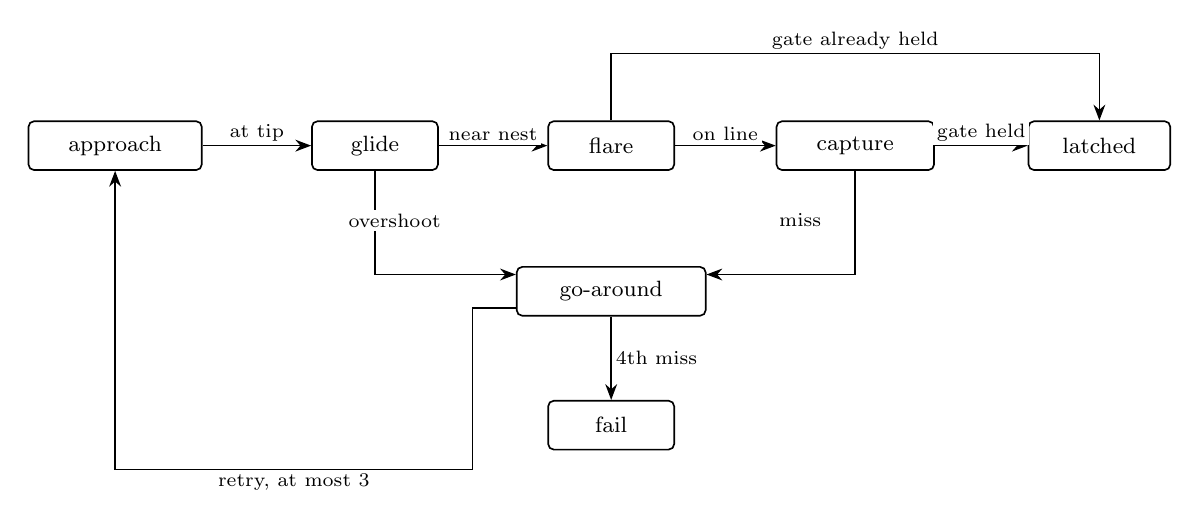
\begin{tikzpicture}
  \node[sm, minimum width=22mm] (tip) at (0,0) {approach};
  \node[sm, minimum width=16mm] (glide) at (3.3,0) {glide};
  \node[sm, minimum width=16mm] (flare) at (6.3,0) {flare};
  \node[sm, minimum width=20mm] (cap) at (9.4,0) {capture};
  \node[sm, minimum width=18mm] (weld) at (12.5,0) {latched};
  \node[sm, minimum width=24mm] (back) at (6.3,-1.85) {go-around};
  \node[sm, minimum width=16mm] (rfail) at (6.3,-3.55) {fail};
  \draw[arr] (tip) -- node[sml, above] {at tip} (glide);
  \draw[arr] (glide) -- node[sml, above] {near nest} (flare);
  \draw[arr] (flare) -- node[sml, above] {on line} (cap);
  \draw[arr] (cap) -- node[sml, above] {gate held} (weld);
  \draw[arr] (flare.north) -- ++(0,0.85) coordinate (top)
    -- node[sml, above] {gate already held} (weld.north |- top) -- (weld.north);
  \draw[arr] (glide.south) |- (back.170);
  \node[sml] at (3.55,-0.95) {overshoot};
  \draw[arr] (cap.south) |- (back.10);
  \node[sml] at (8.7,-0.95) {miss};
  \draw[arr] (back) -- node[sml, right] {4th miss} (rfail);
  \draw[arr] (back.190) -- ++(-0.55,0) coordinate (rw)
    -- ++(0,-2.05) coordinate (rlow)
    -- node[sml, below] {retry, at most 3} (tip.south |- rlow) -- (tip.south);
\end{tikzpicture}

\vspace{2.5mm}
{\footnotesize (b) Rendezvous. The weld is sent as soon as its gate has held, from the flare or from capture.}
\caption{Skill machines for the joint mission. A hoop pass is one sample in the authored opening and a later arrival at the frozen exit. The rendezvous follows the boat centreline. A fourth go-around fails that skill. A hoop failure under \texttt{on\_fail} hold stays armed, so the plan in Fig.~\ref{fig:plan} still starts the rendezvous.}
\label{fig:skills}
\end{figure*}

The upward camera and deck tag 10 remain the nest sensor for the servo and for a pure track. Track holds the upward camera about 1\,m under that tag, using the boat pose as a prediction and the tag as the correction, and it does not weld. The joint mission uses rendezvous, not track, because the sentence asks for a dock.

\section{Demonstrations in the twin}
\label{sec:results}

These are single runs of the behaviours as they stood on one day of simulator time. They are not a Monte Carlo study, and the timed-swim comparison is not a paired trial from identical initial conditions. The timed 8\,m west leg was flown earlier the same day, at a 2\,m/s pace, from a different pose. We report it because it is the failure the LOS change was meant to remove, not as a controlled A/B test.

\subsection{Straight swim}
Table~\ref{tab:swim} summarises three legs. The timed leg was given a 2\,m/s carrot. It passed the 0.35\,m arrival test with 0.34\,m of miss, but it ran up to 1.36\,m off the line while the carrot moved ahead, and the progress gate had already slowed the clock. The two LOS legs were given the 6.2\,m/s cruise number and did not reach it. Both began far from the leg heading and yawed in place before the surge rose. Peak thrust stayed under a quarter of full scale. The 3\,m south leg stopped 0.52\,m off the end and the force-loop settle brought it inside 0.35\,m in about 2\,s. No odometry-consistency reject fired on either LOS run.

\begin{table}[t]
\caption{Straight swims in the Kiwanis twin. ``Off line'' is cross-track for LOS and distance behind the timed carrot for the older guidance. Thrust is the fraction of 144\,N.}
\label{tab:swim}
\centering
\begin{tabular}{lccc}
\toprule
 & Timed 8\,m W & LOS 8\,m W & LOS 3\,m S \\
\midrule
Initial turn & --- & 173$^\circ$ & 122$^\circ$ \\
Duration & 8.1\,s & 8.4\,s & 10.3\,s \\
Off line, max & 1.36\,m & 0.55\,m & 0.52\,m \\
Depth error & --- & 0.16\,m & 0.07\,m \\
Peak thrust & spike$\sim$50\,N & 0.24 & 0.17 \\
Nose, down / up & to $-37^\circ$ & $+4^\circ/-11^\circ$ & $+12^\circ/-7^\circ$ \\
Arrival miss & 0.34\,m & 0.34\,m & 0.35\,m \\
\bottomrule
\end{tabular}
\end{table}

The 50\,N and $-37^\circ$ figures in the last timed column are from the 6.2\,m/s pace on an earlier 8\,m leg, not from the 2\,m/s row's own peak. Both failures belong to the timed reference: too much feedforward at one pace, too little steering force at the other. The table's timed row is the 2\,m/s run. We do not claim the LOS legs are faster. We claim they do not leave the line to chase a carrot, and they do not brake by pitching.

A separate check of the guidance, without ROS, integrates a point hull that can only move along its nose, with the same drag and a rate limit on heading and pitch. Straight legs, a 1\,m initial cross-track error, a depth change, a reverse from past the end, a right-angle corner, and a nose-down bias all arrive inside 0.35\,m. A leg with almost no horizontal length is rejected, because LOS has no direction to steer along.

\subsection{Undock, hoop, rendezvous}
The sentence ``undock, fly through the hoop, and rendezvous with \otterk{}'' produced three steps: detach, hoop, rendezvous. Detach completed. The hoop reported a pass: the closest in-opening sample was 0.10\,m from the authored centre, and the exit miss was 0.42\,m, inside the 0.6\,m gate. The hoop step's thrust interval was 20.9\,s. Rendezvous then ran for 33.6\,s and the latch reported attached. The AUV ended welded, not holding in free swim.

An earlier build of the same day did not complete this chain. A helper added to the shared controller was named the same as a hoop method with a different signature, so every hoop raised a type error a few seconds in and the plan stopped before rendezvous. The helper was renamed, and a unit test now fails if a behaviour class defines a method that belongs to the base controller. We record this because the mission failure was not in the language layer. The plan was already detach, hoop, rendezvous. The state machine ran that plan. The vehicle code crashed inside the second step.

Fig.~\ref{fig:tour} is the latest run of the same sentence. The boat stayed within 0.2\,m of $(-6.3, 0.08, -0.14)$\,m. The hoop log begins at the surface, 0.84\,m from that pose.

\begin{figure*}[t]
\centering
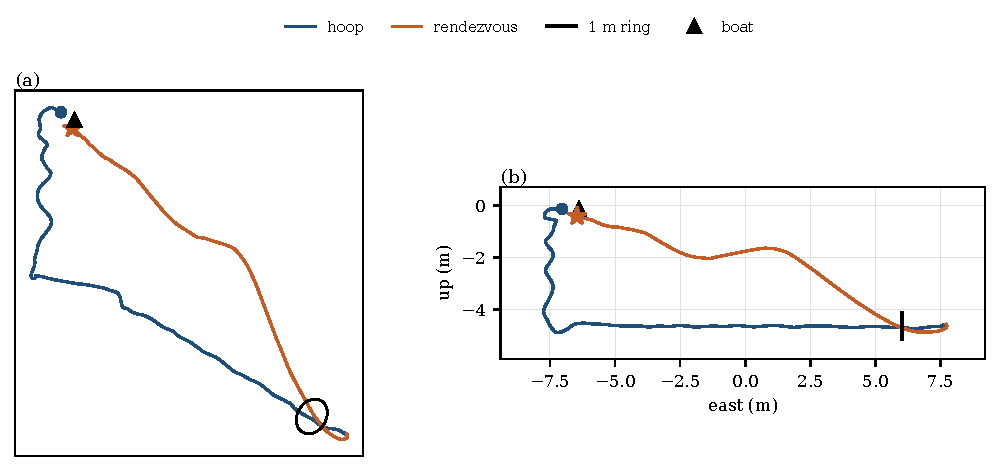
\includegraphics[width=\textwidth]{tour_3d.pdf}
\caption{Latest tour in the Kiwanis twin: the hoop log joined to the rendezvous that took the baton. (a)~Three-dimensional view at equal scale, from the south-east, so east runs down and to the right and a small north offset separates the two legs. (b)~The same track in the east--up plane. The AUV dived beside the boat, levelled at hoop depth, and crossed the 1\,m ring 0.06\,m from its centre. It finished the hoop 1.6\,m farther east. The return climbed along nearly the same vertical plane and latched 31\,s later, 0.28\,m from the logged boat pose and 0.26\,m below it. North offset stayed within 1.03\,m outbound and 0.88\,m on the return. Nose-down pitch reached $55^\circ$ on the dive and $67^\circ$ on the climb, for about 2\,s and under 1\,s, past the $45^\circ$ cruise limit. Peak thrust was 0.05 of full scale on the hoop and 0.06 on the rendezvous.}
\label{fig:tour}
\end{figure*}

\subsection{Rendezvous geometry, separately}
Before the centreline glide, six rendezvous runs on the older point-pursuit terminal included three that orbited 0.2--0.9\,m under the nest before latching. After the change, runs from off the centreline and from a straight approach latched on the first pass, and a deliberate 0.6\,m bias in the boat prior was pulled below 0.1\,m within about a second of the first stern-tag frames. With no injected bias, the vision offset against the simulator boat stayed on the order of a few centimetres to 0.15\,m and was held after the tags left the camera. These runs are the evidence for Section~\ref{sec:mission}'s claim that the hull should fly the line rather than a point under the nest. They are not a full dock-success rate.

\subsection{Logs}
Every behaviour on the shared controller writes a directory per run: a trajectory table in world coordinates, an event log, and a summary (error, saturation, nose limits, speed, distance, verdict). LOS rows add cross-track error, depth off the line, and the speed command. Runs are not overwritten. The summaries above were read back from those records. A single overwritten log had been the previous practice, and it is what made the pace failures harder to compare.

\section{Limitations}
\label{sec:limits}

The lake bed is a bowl, not a survey, and the props have no collision. A pass that clips the real ring would not clip this one. Buoyancy does not depend on the hull's submerged volume beyond the density field. The 0.3\,N trim is a model choice that matches the simulated rest pose; it is not a measured vehicle.

The swim comparison is three legs. The joint mission result is one successful chain after a software fault was fixed. We do not report a success rate over initial headings, boat speeds, or lighting. The boat was not driving a survey during the tour run reported here. Docking against a fast boat is an open case in the earlier kinematic study that chose the rendezvous speed limits.

Coverage, the rendezvous transit out to the glide, and the search pattern still use timed references. The hold behaviour, which is the force loop at a point, still swings the nose tens of degrees at near-zero force. That is the same heading rule that refuses to yaw on a tiny horizontal force, and it is visible in the trajectory logs.

The language layer will still fly whatever typed step the planner emits. The fixed tour is protected by the recognizer. A novel sentence is protected only by the behaviour's own checks: geofence and acceptance tests where they exist, and a busy lock. There is no separate auditor that rejects a plan after the model writes it.

\section{Conclusion}
\label{sec:conclusion}

\CoRAL{} treats a joint lake mission as a sentence over a small set of behaviours, not as a trajectory the language model is free to invent. In the Kiwanis twin the sentence ``undock, fly through the hoop, and rendezvous with the boat'' is detach, then the hoop, then a centreline dock under \otterk{}. The AUV that flies those steps cannot sway. Straight legs therefore use LOS guidance and a surge speed loop, and the timed carrot that used to pull the hull off the line is kept only for curves, holds, and the dock's last metre. One tour run passed the hoop and latched. The next measurements that would change the claim are a repeated tour with the boat underway, and the same LOS law on the lawnmower and on the rendezvous transit.

\balance
\begin{thebibliography}{9}

\bibitem{anand2020}
H.~Anand, ``Coordinated navigation and localization of an autonomous underwater vehicle using an autonomous surface vehicle in the {OpenUAV} simulation framework,'' M.S.\ thesis, Arizona State Univ., Tempe, AZ, USA, Aug.\ 2020. [Online]. Available: \url{https://keep.lib.asu.edu/_flysystem/fedora/c7/233928/Anand_asu_0010N_20290.pdf}

\bibitem{fossen2011}
T.~I. Fossen, \emph{Handbook of Marine Craft Hydrodynamics and Motion Control}. Hoboken, NJ, USA: Wiley, 2011.

\bibitem{lekkas2014}
A.~M. Lekkas and T.~I. Fossen, ``Integral {LOS} path following for curved paths based on a monotone cubic {Hermite} spline parametrization,'' \emph{IEEE J.\ Ocean.\ Eng.}, vol.~39, no.~2, pp.~401--404, Apr.\ 2014.

\bibitem{olson2011}
E.~Olson, ``{AprilTag}: A robust and flexible visual fiducial system,'' in \emph{Proc.\ IEEE Int.\ Conf.\ Robot.\ Autom.\ (ICRA)}, Shanghai, China, 2011, pp.~3400--3407.

\bibitem{meier2015}
L.~Meier, D.~Honegger, and M.~Pollefeys, ``{PX4}: A node-based multithreaded open source robotics framework for deeply embedded platforms,'' in \emph{Proc.\ IEEE Int.\ Conf.\ Robot.\ Autom.\ (ICRA)}, Seattle, WA, USA, 2015, pp.~6235--6240.

\bibitem{koenig2004}
N.~Koenig and A.~Howard, ``Design and use paradigms for {Gazebo}, an open-source multi-robot simulator,'' in \emph{Proc.\ IEEE/RSJ Int.\ Conf.\ Intell.\ Robots Syst.\ (IROS)}, Sendai, Japan, 2004, pp.~2149--2154.

\bibitem{macenski2022}
S.~Macenski, T.~Foote, B.~Gerkey, C.~Lalancette, and W.~Woodall, ``Robot {Operating System 2}: Design, architecture, and uses in the wild,'' \emph{Sci.\ Robot.}, vol.~7, no.~66, p.~eabm6074, May 2022.

\bibitem{hackbarth2015}
A.~Hackbarth, E.~Kreuzer, and E.~Solowjow, ``{HippoCampus}: A micro underwater vehicle for swarm applications,'' in \emph{Proc.\ IEEE/RSJ Int.\ Conf.\ Intell.\ Robots Syst.\ (IROS)}, Hamburg, Germany, 2015, pp.~2258--2263.

\end{thebibliography}

\end{document}
